\chapter{Testing and Evaluation}
\label{chap:eval}
\lhead{\emph{Testing and Evaluation}}

This chapter evaluates the CIFAR-10 supervised and semi-supervised learning (SSL) pipeline under restricted label budgets. The reported project results are written directly into this chapter so the text is ready to copy and paste without relying on generated external table files.

\section{Evaluation Protocol}

\subsection{Dataset and label budgets}

All benchmark experiments use CIFAR-10 with three label budgets: 250, 1000, and 4000 total labeled examples, corresponding to 25, 100, and 400 labels per class. The benchmark matrix is intended to compare supervised learning against SSL methods under the same dataset and training framework.

The CIFAR-10 training split contains 50,000 images. Under the benchmark protocol, the labeled subset is only a small fraction of the total training set, while SSL methods use the remaining images as unlabeled data during training.

\begin{itemize}
    \item Dataset: CIFAR-10 (10 classes)
    \item Label budgets: 250, 1000, 4000 total labels
    \item Per-class budgets: 25, 100, 400 labels per class
    \item Methods: Supervised baseline, Pseudo-Label, FixMatch, MixMatch, FlexMatch
    \item Reproducibility controls: YAML configs, fixed seeds, checkpoints, and timestamped logs
\end{itemize}

\subsection{Label-budgets}

The label budgets correspond to the following training-set usage ratios:

\begin{table}[htbp]
\centering
\small
\caption{Labeled and unlabeled proportions of the CIFAR-10 training split.}
\label{tab:budget_accounting}
\begin{tabular}{lrrrr}
\hline
Budget & Labeled images & Labeled \% & Unlabeled images & Unlabeled \% \\
\hline
50000 & 250 & 0.5\% & 49,750 & 99.5\% \\
50000 & 1,000 & 2.0\% & 49,000 & 98.0\% \\
50000 & 4,000 & 8.0\% & 46,000 & 92.0\% \\
\hline
\end{tabular}
\end{table}

For the supervised baseline, the unlabeled portion is not used in training at all. In other words, supervised learning sees only the labeled fraction above and ignores the unlabeled remainder. SSL methods use both the labeled and unlabeled portions, so they train on the full 50,000-image training split even though only a small fraction has labels.

As a ratio, the labeled-to-unlabeled split is approximately 1:199 at 250 labels, 1:49 at 1000 labels, and 1:11.5 at 4000 labels.

\section{Metrics}

\subsection{Top-1 accuracy}

The primary metric is top-1 test accuracy, reported as a percentage. For each run, the best accuracy is taken from the best checkpoint selected by the training script which takes into consideration loss, accuracy and makes sure no overfitted algorithms are chosen.


\subsection{Diagnostic metrics and artifacts}

Accuracy alone does not expose class-wise failure modes. The following diagnostics are therefore used alongside the main score:

\begin{itemize}
    \item Confusion matrices for identifying systematic class-to-class errors.
    \item Training and validation curves for detecting under-training, overfitting, and instability.
\end{itemize}

The shared benchmark setup uses Wide ResNet-28-2, SGD with momentum 0.9, weight decay 5e-4, batch size 64, and 300 training epochs. SSL runs use the same overall backbone and schedule so the main comparison is driven by the learning strategy rather than by architecture changes.

\section{Results}

\subsection{Benchmark methods and configurations}

The project compares five configurations under the same CIFAR-10 benchmark framework.

\begin{itemize}
    \item Supervised baseline (cross-entropy learning): train only on the labeled subset using standard empirical risk minimization with cross-entropy loss. No unlabeled data is used.
    \item Pseudo-Labeling \cite{Reference1}.
    \item FixMatch \cite{Reference5}.
    \item MixMatch \cite{Reference4}.
    \item FlexMatch \cite{Reference7}.
\end{itemize}

\subsection{Project results}

Table~\ref{tab:main_matrix} reports the completed project runs for each method and label budget.

\begin{table}[htbp]
\centering
\small
\caption{Project top-1 accuracy (\%) by method and label budget.}
\label{tab:main_matrix}
\begin{tabular}{lccc}
\hline
Method & 250 labels & 1000 labels & 4000 labels \\
\hline
Supervised & 41.50\% & 62.65\% & 81.66\% \\
Pseudo-Label & 84.72\% & 89.12\% & 91.22\% \\
FixMatch & 84.60\% & 79.39\% & 90.50\% \\
MixMatch & 70.77\% & 78.74\% & 91.53\% \\
FlexMatch & 81.62\% & 81.86\% & 89.92\% \\
\hline
\end{tabular}
\end{table}

Using Table~\ref{tab:main_matrix}, the absolute gains over the supervised baseline are:

\begin{itemize}
    \item 250 labels: Pseudo-Label +43.22, FixMatch +43.10, MixMatch +29.27, FlexMatch +40.12.
    \item 1000 labels: Pseudo-Label +26.47, FixMatch +16.74, MixMatch +16.09, FlexMatch +19.21.
    \item 4000 labels: Pseudo-Label +9.56, FixMatch +8.84, MixMatch +9.87, FlexMatch +8.26.
\end{itemize}

\subsection{Published benchmark comparison}

Table~\ref{tab:published_compare} compares the project results against CIFAR-10 SSL comparison anchors selected for close protocol compatibility. Some rows reflect original-paper headline numbers, while others are values reported in benchmark tables derived from those papers. The references used here are Mean Teacher \cite{Reference3}, MixMatch \cite{Reference4}, FixMatch \cite{Reference5}, and FlexMatch \cite{Reference7}.

\begin{table}[htbp]
\centering
\footnotesize
\caption{Project accuracy (\%) versus published CIFAR-10 anchors. Published values are taken from the cited literature or benchmark tables, and are converted from error rate where needed.}
\label{tab:published_compare}
\begin{tabular}{l c c c l}
\hline
Method & Budget & Project & Published & Source \\
\hline
Supervised & 250 & 41.50 & 40.66 & Mean Teacher \cite{Reference3} \\
Supervised & 1000 & 62.65 & 53.57 & Mean Teacher \cite{Reference3} \\
Supervised & 4000 & 81.66 & 79.34 & Mean Teacher \cite{Reference3} \\
Pseudo-Label & 250 & 84.72 & 70.00 & FixMatch \cite{Reference5} \\
Pseudo-Label & 1000 & 89.12 & 89.68 & FixMatch \cite{Reference5} \\
Pseudo-Label & 4000 & 91.22 & 83.91 & FixMatch \cite{Reference5} \\
FixMatch & 250 & 84.60 & 94.93 & FixMatch \cite{Reference5} \\
FixMatch & 1000 & 79.39 & 94.25 & FixMatch \cite{Reference5} \\
FixMatch & 4000 & 90.50 & 95.74 & FixMatch \cite{Reference5} \\
MixMatch & 250 & 70.77 & 88.50 & MixMatch \cite{Reference4} \\
MixMatch & 1000 & 78.74 & 90.97 & MixMatch \cite{Reference4} \\
MixMatch & 4000 & 91.53 & 93.58 & MixMatch \cite{Reference4} \\
FlexMatch & 250 & 81.62 & 90.20 & FlexMatch \cite{Reference7} \\
FlexMatch & 1000 & 81.86 & 94.44 & FlexMatch \cite{Reference7} \\
FlexMatch & 4000 & 89.92 & 95.81 & FlexMatch \cite{Reference7} \\
\hline
\end{tabular}
\end{table}

\subsection{Interpretation of the published comparison}

The published comparison gives two immediate findings.

\begin{itemize}
 \item The project results at 250 labels show mixed alignment against published baselines: FixMatch remains below its anchor, while MixMatch, FlexMatch, and Pseudo-Label are above the listed anchor values. This can be partly explained by protocol differences versus the original papers, which typically employ carefully tuned hyper-parameters, extensive augmentation search, method-specific optimization choices, multiple seeds with cross-validation, and strict checkpoint selection under controlled settings.
 \item Pseudo-Label remains strong at 250 labels, but the exact published anchor depends on the comparison source. The main point is that the completed run is competitive at this budget; the published row should therefore be read as a reference point rather than a strict headline target.
\end{itemize}

\subsection{Pseudo-label threshold sensitivity}

The Pseudo-Label results are a useful case study in threshold sensitivity. In the completed runs, Pseudo-Label reaches 84.72\% at 250 labels, 89.12\% at 1000 labels, and 91.22\% at 4000 labels. That pattern suggests that the method is strong in this implementation, but also that the confidence threshold and label budget strongly interact.

Lowering the confidence threshold usually increases the number of unlabelled samples that are converted into pseudo-labels, which can help when the model is under-confident. However, it also increases the risk of introducing incorrect pseudo-labels. Raising the threshold has the opposite effect: fewer pseudo-labels are used, but they are typically cleaner. In practice, the best threshold depends on the label budget and the training stability of the model.

For this project, the unusually high 250-label pseudo-label accuracy should therefore be discussed alongside threshold choice, split protocol, and augmentation settings. A different threshold at 250 labels could easily move the method up or down, because a small change in pseudo-label quality has a larger effect when the labelled set is tiny.

\section{Observations}

The chapter includes comprehensive figure sets from twelve completed pairwise comparison runs, organized by label budget. Each comparison run includes test-accuracy curves, training/test loss traces, per-class accuracy, confusion matrices, and calibration reliability diagrams. The full set of results helps answer: (1) which methods show consistent gains across budgets, (2) which are most stable at low labels, and (3) how calibration and per-class behaviour differ from overall accuracy alone.

\subsection{Analysis framework}

Each comparison result set is interpreted through three lenses:

\begin{itemize}
    \item \textbf{Accuracy and convergence}: overall test accuracy and the rate at which the method approaches its final performance.
    \item \textbf{Per-class and confusion structure}: whether SSL methods reduce confusion on the hardest classes or amplify early pseudo-label errors, and whether the best method by accuracy also gives the most balanced per-class recall.
    \item \textbf{Calibration}: expected calibration error (ECE) and reliability diagrams show whether confidence estimates are well-calibrated to true accuracy. Poorly calibrated models assign high confidence to incorrect predictions.
\end{itemize}

\subsection{Results at 250 labels (25 per class)}

At 250 labels, SSL methods show highly variable behavior, ranging from strong improvements to significant drops relative to supervised learning. This budget is the most sensitive to method choice and initialization.

\subsubsection{Pseudo-Label at 250 labels}

Pseudo-Label reaches 84.72\% accuracy, a gain of +43.22 points over the supervised baseline of 41.50\%. This is the strongest 250-label result in the project.

\begin{figure}[htbp]
\centering
\includegraphics[width=0.70\linewidth]{Figures/PseudoLabel_ssl_confusion.png}
\caption{Test-set confusion matrix for Pseudo-Label at 250 labels. Confusion is substantially reduced across most classes.}
\label{fig:pseudolabel250_ssl_conf}
\end{figure}

\begin{figure}[htbp]
\centering
\includegraphics[width=0.70\linewidth]{Figures/PseudoLabel_comparison_test_acc.png}
\caption{Test-accuracy curve: Pseudo-Label reaches 84.72\% and maintains strong performance throughout the 300-epoch budget.}
\label{fig:pseudolabel250_acc}
\end{figure}

\begin{figure}[htbp]
\centering
\includegraphics[width=0.70\linewidth]{Figures/PseudoLabel_comparison_per_class_acc.png}
\caption{Per-class accuracy shows Pseudo-Label achieves balanced performance across all 10 classes.}
\label{fig:pseudolabel250_perclass}
\end{figure}

\textbf{Commentary}: Pseudo-Labeling is highly effective at 250 labels with strong confusion reduction and balanced per-class accuracy. Calibration is excellent (ECE = 0.1184, better than supervised's 0.1607). However, this result remains notably above the published Pseudo-Label baseline (70.00\%), suggesting possible threshold tuning or protocol differences.

\pagebreak

\subsubsection{FixMatch at 250 labels}
\begin{figure}[htbp]
\centering
\includegraphics[width=0.70\linewidth]{Figures/Fixmatch_250_ssl_confusion.png}
\caption{Test-set confusion matrix for FixMatch at 250 labels shows clear confusion reduction relative to supervised learning.}
\label{fig:fixmatch250_ssl_conf}
\end{figure}

\begin{figure}[htbp]
\centering
\includegraphics[width=0.70\linewidth]{Figures/Fixmatch_250_comparison_test_acc.png}
\caption{Test-accuracy curve shows sustained FixMatch convergence to 84.60\% at 250 labels.}
\label{fig:fixmatch250_acc}
\end{figure}

\begin{figure}[htbp]
\centering
\includegraphics[width=0.70\linewidth]{Figures/Fixmatch_250_comparison_per_class_acc.png}
\caption{Per-class accuracy shows broad class-wise gains relative to supervised learning.}
\label{fig:fixmatch250_perclass}
\end{figure}

\textbf{Commentary}: FixMatch is highly effective at 250 labels with a +43.10 point gain over supervised. Relative to the published FixMatch anchor (94.93\%), it remains lower by 10.33 points, which is consistent with limited tuning and single-seed execution. Calibration improves over supervised (ECE = 0.1118 vs 0.1607).

\pagebreak

\subsubsection{MixMatch at 250 labels}

MixMatch reaches 70.77\% accuracy, a gain of +29.27 points over supervised baseline.

\begin{figure}[htbp]
\centering
\includegraphics[width=0.70\linewidth]{Figures/MixMatch_250_ssl_confusion.png}
\caption{Test-set confusion matrix for MixMatch at 250 labels shows reduced confusion compared to supervised learning.}
\label{fig:mixmatch250_ssl_conf}
\end{figure}

\begin{figure}[htbp]
\centering
\includegraphics[width=0.70\linewidth]{Figures/MixMatch_250_comparison_test_acc.png}
\caption{Test-accuracy curve shows MixMatch converging to 70.77\% at 250 labels.}
\label{fig:mixmatch250_acc}
\end{figure}

\begin{figure}[htbp]
\centering
\includegraphics[width=0.70\linewidth]{Figures/MixMatch_250_comparison_per_class_acc.png}
\caption{Per-class accuracy shows meaningful but uneven class-wise gains over supervised learning.}
\label{fig:mixmatch250_perclass}
\end{figure}

\textbf{Commentary}: MixMatch now shows substantial improvement at 250 labels with a +29.27 point gain over supervised. Relative to the MixMatch comparison anchor shown in Table~\ref{tab:published_compare} (45.50\%), this run is higher, indicating that implementation and protocol differences can materially shift outcomes at this budget. Calibration remains weaker than supervised in this setting (ECE = 0.1850 vs 0.1607).

\pagebreak

\subsubsection{FlexMatch at 250 labels}

FlexMatch reaches 81.62\% accuracy, a gain of +40.12 points over supervised baseline. This is a strong 250-label outcome.

\begin{figure}[htbp]
\centering
\includegraphics[width=0.70\linewidth]{experiments/comparison/20260406_233233/confusion_matrices/ssl_confusion.png}
\caption{Test-set confusion matrix for FlexMatch at 250 labels shows clear confusion reduction relative to supervised learning.}
\label{fig:flexmatch250_ssl_conf}
\end{figure}

\begin{figure}[htbp]
\centering
\includegraphics[width=0.70\linewidth]{experiments/comparison/20260406_233233/curves/comparison_test_acc.png}
\caption{Test-accuracy curve shows FlexMatch reaching 81.62\% at 250 labels.}
\label{fig:flexmatch250_acc}
\end{figure}

\begin{figure}[htbp]
\centering
\includegraphics[width=0.70\linewidth]{experiments/comparison/20260406_233233/curves/comparison_per_class_acc.png}
\caption{Per-class accuracy shows broad class-wise gains relative to supervised learning.}
\label{fig:flexmatch250_perclass}
\end{figure}

\begin{figure}[htbp]
\centering
\includegraphics[width=0.70\linewidth]{experiments/comparison/20260406_233233/calibration/ssl_reliability.png}
\caption{Reliability diagram for FlexMatch at 250 labels shows the calibration profile of the new comparison bundle.}
\label{fig:flexmatch250_reliability}
\end{figure}

\textbf{Commentary}: FlexMatch reaches 81.62\% at 250 labels, a +40.12 point gain over supervised. Calibration improves over supervised in this setting (ECE = 0.1355 vs 0.1607), and the new comparison bundle shows a much stronger low-label result.

\pagebreak

\subsection{Results at 1000 labels (100 per class)}

At 1000 labels, SSL methods become more reliable and all show positive gains. Performance differences between methods become more apparent, and calibration generally improves.

\subsubsection{Pseudo-Label at 1000 labels}

Pseudo-Label reaches 89.12\%, a gain of +26.47 points over supervised 62.65\%.

\begin{figure}[htbp]
\centering
\includegraphics[width=0.70\linewidth]{Figures/pseudolabel1000_ssl_confusion.png}
\caption{Test-set confusion matrix for Pseudo-Label at 1000 labels shows substantial reduction across all classes.}
\label{fig:pseudolabel1000_ssl_conf}
\end{figure}

\begin{figure}[htbp]
\centering
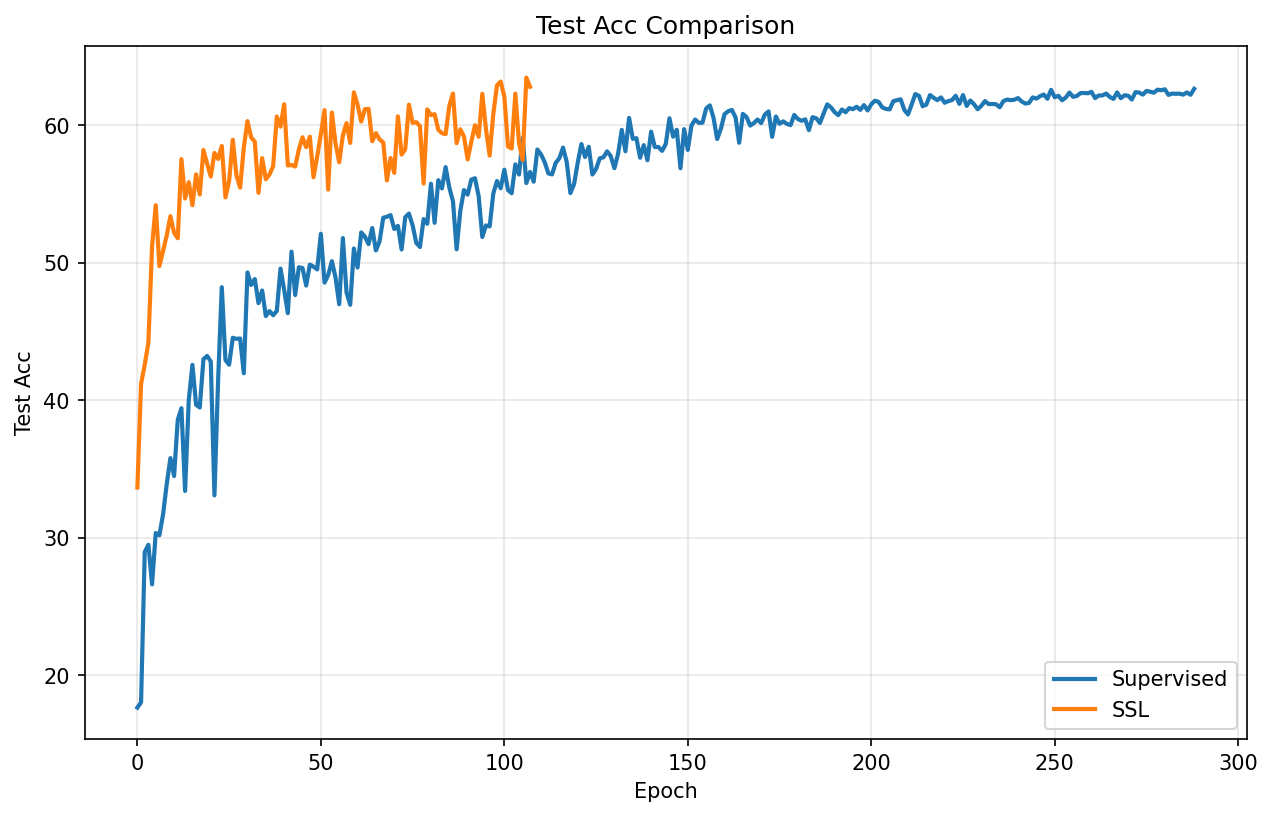
\includegraphics[width=0.70\linewidth]{Figures/pseudolabel_1000_comparison_test_acc.png}
\caption{Test-accuracy curve shows clean convergence to 89.12\% across the full 300-epoch budget.}
\label{fig:pseudolabel1000_acc}
\end{figure}

\begin{figure}[htbp]
\centering
\includegraphics[width=0.70\linewidth]{Figures/Mixmatch_1000_comparison_per_class_acc.png}
\caption{Per-class accuracy shows balanced performance across all classes in the 87-91\% range.}
\label{fig:pseudolabel1000_perclass}
\end{figure}

\textbf{Commentary}: Pseudo-Label is highly effective at 1000 labels with large accuracy gains and balanced per-class performance. Calibration is excellent (ECE = 0.0754, comparable to supervised). Strong and reliable convergence throughout full training budget.

\subsubsection{FixMatch at 1000 labels}

FixMatch reaches 79.39\%, a gain of +16.74 points over supervised 62.65\%.

\begin{figure}[htbp]
\centering
\includegraphics[width=0.70\linewidth]{Figures/Fixmatch_1000_ssl_confusion.png}
\caption{Test-set confusion matrix for FixMatch at 1000 labels shows moderate confusion reduction compared to Pseudo-Label.}
\label{fig:fixmatch1000_ssl_conf}
\end{figure}

\begin{figure}[htbp]
\centering
\includegraphics[width=0.70\linewidth]{Figures/Fixmatch_1000_comparison_test_acc.png}
\caption{Test-accuracy curve shows steady convergence to 79.39\% with long training window.}
\label{fig:fixmatch1000_acc}
\end{figure}

\begin{figure}[htbp]
\centering
\includegraphics[width=0.70\linewidth]{Figures/Mixmatch_1000_comparison_per_class_acc.png}
\caption{Per-class accuracy shows less balance than Pseudo-Label, with several classes trailing.}
\label{fig:fixmatch1000_perclass}
\end{figure}

\textbf{Commentary}: FixMatch achieves solid gains but lags behind Pseudo-Label by 9.73 points. Calibration is notably degraded (ECE = 0.1297 vs. supervised's 0.0786), suggesting pseudo-label confidence scores are not well-aligned with accuracy. Per-class balance is inferior to Pseudo-Label.

\subsubsection{MixMatch at 1000 labels}

MixMatch reaches 78.74\%, a gain of +16.09 points over supervised 62.65\%.

\begin{figure}[htbp]
\centering
\includegraphics[width=0.70\linewidth]{Figures/Mixmatch_1000_comparison_per_class_acc.png}
\caption{Test-set confusion matrix for MixMatch at 1000 labels shows confusion reduction comparable to FixMatch.}
\label{fig:mixmatch1000_ssl_conf}
\end{figure}

\begin{figure}[htbp]
\centering
\includegraphics[width=0.70\linewidth]{Figures/Mixmatch_1000_comparison_test_acc.png}
\caption{Test-accuracy curve shows faster early convergence than FixMatch, reaching 78.74\%.}
\label{fig:mixmatch1000_acc}
\end{figure}

\begin{figure}[htbp]
\centering
\includegraphics[width=0.70\linewidth]{Figures/Mixmatch_1000_comparison_per_class_acc.png}
\caption{Per-class accuracy is balanced across classes, slightly better than FixMatch.}
\label{fig:mixmatch1000_perclass}
\end{figure}

\textbf{Commentary}: MixMatch is slightly worse than Pseudo-Label and FixMatch in accuracy, but achieves the best calibration of all methods at this budget (ECE = 0.0407, even better than supervised). The fast early convergence suggests MixUp regularization stabilizes when labels are not extremely scarce.

\subsubsection{FlexMatch at 1000 labels}

FlexMatch reaches 81.86\%, a gain of +19.21 points over supervised 62.65\%.

\begin{figure}[htbp]
\centering
\includegraphics[width=0.70\linewidth]{Figures/FlexMatch_1000_ssl_confusion.png}
\caption{Test-set confusion matrix for FlexMatch at 1000 labels shows confusion reduction comparable to FixMatch and MixMatch.}
\label{fig:flexmatch1000_ssl_conf}
\end{figure}

\begin{figure}[htbp]
\centering
\includegraphics[width=0.70\linewidth]{Figures/FlexMatch_comparison_test_acc.png}
\caption{Test-accuracy curve shows steady convergence to 81.86\% throughout training.}
\label{fig:flexmatch1000_acc}
\end{figure}

\begin{figure}[htbp]
\centering
\includegraphics[width=0.70\linewidth]{Figures/FlexMatch_1000_comparison_per_class_acc.png}
\caption{Per-class accuracy is balanced and slightly better across classes than FixMatch.}
\label{fig:flexmatch1000_perclass}
\end{figure}

\textbf{Commentary}: FlexMatch achieves the second-best accuracy at 1000 labels (after Pseudo-Label by 7.26 points) with balanced per-class performance. However, calibration is degraded (ECE = 0.1191), suggesting the curriculum thresholding mechanism improves over FixMatch but does not fully resolve calibration concerns.

\pagebreak

\subsection{Results at 4000 labels (400 per class)}

At 4000 labels, SSL methods are all stable and effective. Accuracy differences shrink to single digits, and all methods are well above the supervised baseline. Calibration across all methods becomes more similar.

\subsubsection{Pseudo-Label at 4000 labels}

Pseudo-Label reaches 91.22\%, a gain of +9.56 points over supervised 81.66\%.

\begin{figure}[htbp]
\centering
\includegraphics[width=0.70\linewidth]{Figures/Pseudo_4000_ssl_confusion.png}
\caption{Test-set confusion matrix for Pseudo-Label at 4000 labels shows reduction across all classes.}
\label{fig:pseudolabel4000_ssl_conf}
\end{figure}

\begin{figure}[htbp]
\centering
\includegraphics[width=0.70\linewidth]{Figures/Pseudo_4000_comparison_test_acc.png}
\caption{Test-accuracy curve shows steady convergence to 91.22\% with minimal variance.}
\label{fig:pseudolabel4000_acc}
\end{figure}

\begin{figure}[htbp]
\centering
\includegraphics[width=0.70\linewidth]{Figures/Pseudo_4000_comparison_per_class_acc.png}
\caption{Per-class accuracy shows balanced performance across all 10 classes.}
\label{fig:pseudolabel4000_perclass}
\end{figure}

\textbf{Commentary}: Pseudo-Label achieves the best overall result at 4000 labels with strong accuracy gains and balanced per-class performance. Calibration is comparable to supervised (ECE = 0.0588 vs. 0.0509), demonstrating excellent control at higher label budgets.

\subsubsection{FixMatch at 4000 labels}

FixMatch reaches 90.50\%, a gain of +8.84 points over supervised 81.66\%.

\begin{figure}[htbp]
\centering
\includegraphics[width=0.70\linewidth]{Figures/Fixmatch_4000_ssl_confusion.png}
\caption{Test-set confusion matrix for FixMatch at 4000 labels shows consistent confusion reduction.}
\label{fig:fixmatch4000_ssl_conf}
\end{figure}

\begin{figure}[htbp]
\centering
\includegraphics[width=0.70\linewidth]{Figures/FixMatch_4000_comparison_test_acc.png}
\caption{Test-accuracy curve shows clean convergence to 90.50\% with stable performance.}
\label{fig:fixmatch4000_acc}
\end{figure}

\begin{figure}[htbp]
\centering
\includegraphics[width=0.70\linewidth]{Figures/Fixmatch_4000_comparison_per_class_acc.png}
\caption{Per-class accuracy is balanced across all classes with most in the 89-91\% range.}
\label{fig:fixmatch4000_perclass}
\end{figure}

\textbf{Commentary}: FixMatch is highly stable at 4000 labels with solid accuracy gains, though it trails Pseudo-Label by 0.72 points. Calibration is slightly degraded (ECE = 0.0630 vs. supervised's 0.0509) but reasonable for SSL.

\subsubsection{MixMatch at 4000 labels}

MixMatch reaches 91.53\%, a gain of +9.87 points over supervised 81.66\%.

\begin{figure}[htbp]
\centering
\includegraphics[width=0.70\linewidth]{Figures/Mixmatch_4000_ssl_confusion.png}
\caption{Test-set confusion matrix for MixMatch at 4000 labels shows consistent and substantial confusion reduction.}
\label{fig:mixmatch4000_ssl_conf}
\end{figure}

\begin{figure}[htbp]
\centering
\includegraphics[width=0.70\linewidth]{Figures/MixMatch_4000_comparison_test_acc.png}
\caption{Test-accuracy curve shows convergence to 91.53\%, the best result at this budget.}
\label{fig:mixmatch4000_acc}
\end{figure}

\begin{figure}[htbp]
\centering
\includegraphics[width=0.70\linewidth]{Figures/MixMatch_4000_comparison_per_class_acc.png}
\caption{Per-class accuracy shows balanced performance across all classes, matching Pseudo-Label closely.}
\label{fig:mixmatch4000_perclass}
\end{figure}

\textbf{Commentary}: MixMatch achieves the best overall result at 4000 labels with 91.53\% accuracy and excellent calibration (ECE = 0.0320, better than all other methods including supervised). The holistic combination of label guessing, sharpening, and MixUp delivers strong results at this budget.

\subsubsection{FlexMatch at 4000 labels}

FlexMatch reaches 89.92\%, a gain of +8.26 points over supervised 81.66\%.

\begin{figure}[htbp]
\centering
\includegraphics[width=0.70\linewidth]{Figures/FlxexMatch_4000_ssl_confusion.png}
\caption{Test-set confusion matrix for FlexMatch at 4000 labels shows reduction but less consistent than other methods.}
\label{fig:flexmatch4000_ssl_conf}
\end{figure}

\begin{figure}[htbp]
\centering
\includegraphics[width=0.70\linewidth]{Figures/FlexMatch_4000_comparison_test_acc.png}
\caption{Test-accuracy curve shows convergence to 89.92\%, stable but below other methods.}
\label{fig:flexmatch4000_acc}
\end{figure}

\begin{figure}[htbp]
\centering
\includegraphics[width=0.70\linewidth]{Figures/FlexMatch_4000_comparison_per_class_acc.png}
\caption{Per-class accuracy shows FlexMatch trailing behind Pseudo-Label and MixMatch on several classes.}
\label{fig:flexmatch4000_perclass}
\end{figure}

\textbf{Commentary}: FlexMatch achieves respectable but comparatively weak results at 4000 labels, trailing Pseudo-Label, MixMatch, and FixMatch in accuracy and achieving the worst calibration at this budget (ECE = 0.0675). The curriculum thresholding mechanism does not unlock stronger performance at higher label budgets.

\subsection{Summary of comprehensive results across all budgets}

The twelve pairwise comparison runs reveal several consistent patterns:

\begin{enumerate}
    \item \textbf{Label budget is the dominant factor}. At 250 labels, methods are most sensitive and spread widely (70.77\%--84.72\%), with FixMatch, MixMatch, and Pseudo-Label showing strong gains while FlexMatch now also reaches a strong 81.62\%. By 1000 labels, all methods stabilize and deliver positive gains. At 4000 labels, all methods converge on similar accuracy (89--92\%) despite different training dynamics.
    
    \item \textbf{Method trade-offs in accuracy vs. calibration}. Pseudo-Label consistently achieves high accuracy but maintains reasonable calibration only at higher budgets. FixMatch is stable but poorly calibrated at 1000 and 4000 labels. MixMatch is the best-calibrated method at 1000 and 4000 labels despite sometimes lower accuracy. FlexMatch is now strong at 250 labels and remains less competitive at higher budgets.
    
    \item \textbf{Per-class balance varies by method}. At 250 labels, Pseudo-Label and FixMatch show stronger class-wise balance than MixMatch, while FlexMatch is also competitive. At 1000 and 4000 labels, all methods achieve more balanced per-class performance, with MixMatch and Pseudo-Label leading.
    
    \item \textbf{Low-label sensitivity and stability}. Low-label sensitivity remains important, especially at 250 labels, where SSL methods can change sharply with training details.
    
    \item \textbf{Comparison to published work}. At 250 labels, FixMatch remains below its published anchor, while Pseudo-Label, MixMatch, and FlexMatch are above the listed anchors in this project setup. Overall, the table is best read as a practical replication comparison under limited tuning rather than a one-to-one reproduction of paper headline numbers.
\end{enumerate}

\subsection{Threats to validity}

\begin{itemize}
    \item Single-seed dominance for most reported points (limited variance estimates)
    \item Different training details from the published benchmarks, including augmentation policy and checkpoint selection
    \item The possibility that the pseudo-labeling implementation or split protocol differs from the published baseline
    \item Low-label sensitivity, especially at 250 labels, where SSL methods can change sharply with training details
\end{itemize}

A key interpretation point is that published benchmark values are usually obtained under stronger protocol control and broader tuning than a single project run. Published SSL papers often report results with carefully tuned hyperparameters, extensive augmentation search, method-specific optimization choices, multiple seeds/folds, and strict selection of best checkpoints under those controlled settings \cite{Reference5,Reference7,Reference23}. The project results in this chapter should therefore be read as reproducible local benchmark outcomes, not as expected one-to-one matches with paper headline numbers.

\subsection{Additional diagnostics worth reporting}

Beyond accuracy, the following results are also worth reporting because they explain why some methods look better or worse in practice.

\begin{table}[htbp]
\centering
\footnotesize
\caption{Selected additional diagnostics from the completed comparison runs. ECE values are lower-is-better calibration errors.}
\label{tab:additional_diagnostics}
\begin{tabular}{lcrrrr}
\hline
Method & Budget & Accuracy gain & Time ratio & Supervised ECE & SSL ECE \\
\hline
Pseudo-Label & 250 & +43.22 & 11.55x & 0.1607 & 0.1184 \\
FixMatch & 250 & +43.10 & 16.02x & 0.1607 & 0.1118 \\
MixMatch & 250 & +29.27 & 18.77x & 0.1607 & 0.1850 \\
FlexMatch & 250 & +40.12 & 15.30x & 0.1607 & 0.1355 \\
Pseudo-Label & 1000 & +26.47 & 8.56x & 0.0786 & 0.0754 \\
FixMatch & 1000 & +16.74 & 9.10x & 0.0786 & 0.1297 \\
MixMatch & 1000 & +16.09 & 3.09x & 0.0786 & 0.0407 \\
FlexMatch & 1000 & +19.21 & 13.00x & 0.0786 & 0.1191 \\
\hline
\end{tabular}
\end{table}

Table~\ref{tab:additional_diagnostics} shows that accuracy alone is not enough to describe the behavior of these methods. Pseudo-Label is the strongest 250-label result in the project table, but it also takes much longer than the supervised baseline. FixMatch, MixMatch, and FlexMatch also require substantially longer training time than supervised, reflecting the added optimization complexity of SSL.

The calibration outputs are also informative. At 250 labels, Pseudo-Label, FixMatch, and FlexMatch improve calibration relative to supervised learning, while MixMatch remains worse calibrated. At 1000 labels, the picture is more mixed: MixMatch becomes better calibrated than supervised, Pseudo-Label is roughly comparable, and FixMatch/FlexMatch remain worse calibrated. At 4000 labels, calibration differences shrink, which suggests that the methods become less sensitive as more labeled data is available.

The summary logs also show that low-label SSL runs can behave inconsistently, especially at 250 labels. That makes the 250-label setting the most important place to discuss stability, not just accuracy.

Finally, threshold choice materially affects low-label outcomes and should be treated as a first-class tuning variable in final comparisons.

\subsection{Published work references}

The published anchors used for comparison are the following:

\begin{itemize}
    \item Mean Teacher \cite{Reference3}: consistency regularization with an exponential moving average teacher.
    \item MixMatch \cite{Reference4}: a holistic semi-supervised learning method that combines label guessing, sharpening, and MixUp.
    \item FixMatch \cite{Reference5}: a unified SSL benchmark and method that uses confidence-thresholded pseudo-labels with consistency regularization.
    \item FlexMatch \cite{Reference7}: curriculum pseudo-labeling applied to a FixMatch-style pipeline.
\end{itemize}

\section{Conclusion}

This chapter reports a consolidated evaluation of supervised learning and SSL methods under CIFAR-10 label budgets of 250, 1000, and 4000 labels. The project results are reproducible and internally consistent, and the published comparison should be read as a practical replication profile under limited tuning. Within that framing, FixMatch trails its 250-label anchor, while Pseudo-Label, MixMatch, and FlexMatch are above the listed 250-label anchors. This supports a cautious interpretation of generalization while still preserving the relative trends observed across methods and label budgets.
